\documentclass[journal,12pt]{IEEEtran}
\usepackage{longtable}
\usepackage{setspace}
\usepackage{gensymb}
\singlespacing
\usepackage[cmex10]{amsmath}
\newcommand\myemptypage{
	\null
	\thispagestyle{empty}
	\addtocounter{page}{-1}
	\newpage
}
\usepackage{amsthm}
\usepackage{mdframed}
\usepackage{mathrsfs}
\usepackage{txfonts}
\usepackage{stfloats}
\usepackage{bm}
\usepackage{cite}
\usepackage{cases}
\usepackage{subfig}

\usepackage{longtable}
\usepackage{multirow}

\usepackage{tikz}
\usetikzlibrary{automata, positioning, arrows}

\usepackage{enumitem}
\usepackage{mathtools}
\usepackage{steinmetz}
\usepackage{tikz}
\usepackage{circuitikz}
\usepackage{verbatim}
\usepackage{tfrupee}
\usepackage[breaklinks=true]{hyperref}
\usepackage{graphicx}
\usepackage{tkz-euclide}

\usetikzlibrary{calc,math}
\usepackage{listings}
\usepackage{color}                                            %%
\usepackage{array}                                            %%
\usepackage{longtable}                                        %%
\usepackage{calc}                                             %%
\usepackage{multirow}                                         %%
\usepackage{hhline}                                           %%
\usepackage{ifthen}                                           %%
\usepackage{lscape}     
\usepackage{multicol}
\usepackage{chngcntr}

\DeclareMathOperator*{\Res}{Res}

\renewcommand\thesection{\arabic{section}}
\renewcommand\thesubsection{\thesection.\arabic{subsection}}
\renewcommand\thesubsubsection{\thesubsection.\arabic{subsubsection}}

\renewcommand\thesectiondis{\arabic{section}}
\renewcommand\thesubsectiondis{\thesectiondis.\arabic{subsection}}
\renewcommand\thesubsubsectiondis{\thesubsectiondis.\arabic{subsubsection}}


\hyphenation{op-tical net-works semi-conduc-tor}
\def\inputGnumericTable{}                                 %%

\lstset{
	%language=C,
	frame=single, 
	breaklines=true,
	columns=fullflexible
}
\begin{document}
	\onecolumn
	
	\newtheorem{theorem}{Theorem}[section]
	\newtheorem{problem}{Problem}
	\newtheorem{proposition}{Proposition}[section]
	\newtheorem{lemma}{Lemma}[section]
	\newtheorem{corollary}[theorem]{Corollary}
	\newtheorem{example}{Example}[section]
	\newtheorem{definition}[problem]{Definition}
	
	\newcommand{\BEQA}{\begin{eqnarray}}
		\newcommand{\EEQA}{\end{eqnarray}}
	\newcommand{\define}{\stackrel{\triangle}{=}}
	\bibliographystyle{IEEEtran}
	\raggedbottom
	\setlength{\parindent}{0pt}
	\providecommand{\mbf}{\mathbf}
	\providecommand{\pr}[1]{\ensuremath{\Pr\left(#1\right)}}
	\providecommand{\qfunc}[1]{\ensuremath{Q\left(#1\right)}}
	\providecommand{\sbrak}[1]{\ensuremath{{}\left[#1\right]}}
	\providecommand{\lsbrak}[1]{\ensuremath{{}\left[#1\right.}}
	\providecommand{\rsbrak}[1]{\ensuremath{{}\left.#1\right]}}
	\providecommand{\brak}[1]{\ensuremath{\left(#1\right)}}
	\providecommand{\lbrak}[1]{\ensuremath{\left(#1\right.}}
	\providecommand{\rbrak}[1]{\ensuremath{\left.#1\right)}}
	\providecommand{\cbrak}[1]{\ensuremath{\left\{#1\right\}}}
	\providecommand{\lcbrak}[1]{\ensuremath{\left\{#1\right.}}
	\providecommand{\rcbrak}[1]{\ensuremath{\left.#1\right\}}}
	\theoremstyle{remark}
	\newtheorem{rem}{Remark}
	\newcommand{\sgn}{\mathop{\mathrm{sgn}}}
	\providecommand{\abs}[1]{\left\vert#1\right\vert}
	\providecommand{\res}[1]{\Res\displaylimits_{#1}} 
	\providecommand{\norm}[1]{\left\lVert#1\right\rVert}
	%\providecommand{\norm}[1]{\lVert#1\rVert}
	\providecommand{\mtx}[1]{\mathbf{#1}}
	\providecommand{\mean}[1]{E\left[ #1 \right]}
	\providecommand{\fourier}{\overset{\mathcal{F}}{ \rightleftharpoons}}
	%\providecommand{\hilbert}{\overset{\mathcal{H}}{ \rightleftharpoons}}
	\providecommand{\system}{\overset{\mathcal{H}}{ \longleftrightarrow}}
	%\newcommand{\solution}[2]{\textbf{Solution:}{#1}}
	\newcommand{\solution}{\noindent \textbf{Solution: }}
	\newcommand{\cosec}{\,\text{cosec}\,}
	\providecommand{\dec}[2]{\ensuremath{\overset{#1}{\underset{#2}{\gtrless}}}}
	\newcommand{\myvec}[1]{\ensuremath{\begin{pmatrix}#1\end{pmatrix}}}
	\newcommand{\mydet}[1]{\ensuremath{\begin{vmatrix}#1\end{vmatrix}}}
	\numberwithin{equation}{subsection}
	\makeatletter
	\@addtoreset{figure}{problem}
	\makeatother
	\let\StandardTheFigure\thefigure
	\let\vec\mathbf
	\renewcommand{\thefigure}{\theproblem}
	\def\putbox#1#2#3{\makebox[0in][l]{\makebox[#1][l]{}\raisebox{\baselineskip}[0in][0in]{\raisebox{#2}[0in][0in]{#3}}}}
	\def\rightbox#1{\makebox[0in][r]{#1}}
	\def\centbox#1{\makebox[0in]{#1}}
	\def\topbox#1{\raisebox{-\baselineskip}[0in][0in]{#1}}
	\def\midbox#1{\raisebox{-0.5\baselineskip}[0in][0in]{#1}}
	\vspace{3cm}
	\title{Assignment 15}
	\author{Vimal K B - AI20MTECH12001}
	\maketitle
	\bigskip
	\renewcommand{\thefigure}{\theenumi}
	\renewcommand{\thetable}{\theenumi}
	%
	Download the latex-tikz codes from 
	%
	\begin{lstlisting}
		https://github.com/vimalkb007/EE5609/tree/master/Assignment_15
	\end{lstlisting}
	\section{\textbf{Problem}}
	(UGC-dec2018,106) : \\
	%
	Consider a Markov chain with transition probability matrix $\vec{P}$ given by
	\begin{align}
		P=\myvec{\frac{1}{2} & \frac{1}{2} & 0 \\
			0 & \frac{1}{2} & \frac{1}{2} \\
			\frac{1}{3} & \frac{1}{3} & \frac{1}{3}} \nonumber
	\end{align}
	For any two states $i$ and $j$, let $p^{n}_{ij}$ denote the n-stp transition probability of going from $i$ to $j$. Identify the correct statements
	\begin{enumerate}
		\item $\lim_{n \to \infty} p^{n}_{11} = \frac{2}{9}$
		\item $\lim_{n \to \infty} p^{n}_{21} = 0$
		\item $\lim_{n \to \infty} p^{n}_{32} = \frac{1}{3}$
		\item $\lim_{n \to \infty} p^{n}_{13} = \frac{1}{3}$
	\end{enumerate}
	
	\section{\textbf{Definition and Result used}}
	\begin{longtable}{|l|l|}
		\hline
		\multirow{3}{*}{Irreducible Markov Chain} 
		& \\
		& A Markov chain is $\textbf{irreducible}$ if all the states communicate with each other,\\
		& i.e., if there is only one communication class.\\
		&\\
		\hline
		\multirow{3}{*}{Aperiodic Markov Chain} & \\
		& If there is a self-transition in the chain ($p^{ii}>0$ for some i), then the chain is\\
		& called as $\textbf{aperiodic}$\\
		& \\
		\hline
		\multirow{3}{*}{Stationary Distribution} & \\
		& A stationary distribution of a Markov chain is a probability distribution that\\
		& remains unchanged in the Markov chain as time progresses. Typically, it is\\
		& represented as a row vector $\Vec{\pi}$ whose entries are probabilities summing to 1,\\ 
		& and given transition matrix $\textbf{P}$, it satisfies\\
		& \\
		&  \qquad \qquad  \qquad$\Vec{\pi} = \Vec{\pi} \textbf{P}$\\
		& \\
		\hline
	\end{longtable}
	\newpage
	\section{\textbf{Solution}}
	\begin{longtable}{|l|l|}
		\hline
		\multirow{3}{*}{Drawing Transition diagram} 
		& \\
		& 
		
		$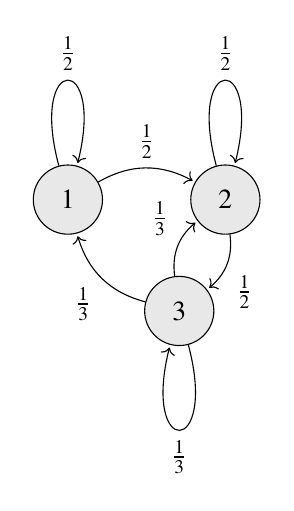
\begin{tikzpicture}[shorten >=1pt,node distance=2cm, scale =3, auto]
			\tikzstyle{every state}=[fill={rgb:black,1;white,10}]
			
			\node[state]   (q_1)                          {$1$};
			\node[state]   (q_2)  [right of=q_1]          {$2$};
			\node[state]   (q_3)  [below right of=q_1]          {$3$};
			
			\path[->]
			(q_1) edge [loop above] node {$\frac{1}{2}$}    (   )
			edge [bend left]  node {$\frac{1}{2}$}    (q_2)
			(q_2) edge [bend left]  node {$\frac{1}{2}$}    (q_3)
			edge [loop above] node {$\frac{1}{2}$}    ()
			(q_3) edge [bend left]  node {$\frac{1}{3}$}    (q_2)
			edge [bend left]  node {$\frac{1}{3}$}    (q_1)
			edge [loop below] node {$\frac{1}{3}$}    ();
		\end{tikzpicture}$
		
		\\  
		&\\
		&\\
		\hline
		\multirow{3}{*}{Checking whether the  } & \\
		& Here,\\chain is Irreducible
		& All the states are accessible to one another. \\and Aperiodic
		& $\implies$ They are in the same communication class. So, it is Irreducible.\\
		& \\
		& There exists the non- zero self-transition, which means that the chain \\
		& is Aperiodic.\\
		&\\ 
		& We know that if the Markov Chain is irreducible and aperiodic then \\
		& \qquad \qquad \qquad $\Vec{\pi}_{j} = \lim_{n \to \infty}P\{X_{n} = j\}$, $j = 1,...,N$ \\
		& These are the stationary probabilities. \\
		&\\
		\hline
		\multirow{3}{*}{Finding the Stationary} & \\
		& Stationary Probability can be represented as\\Probability Distributions
		& \qquad \qquad \qquad $\Vec{\pi} = \Vec{\pi} \vec{P}$\\
		& \\
		& \qquad $\implies$ $\myvec{v_{1}&&v_{2}&&v_{3}} = \myvec{v_{1}&&v_{2}&&v_{3}}\vec{P}$ \\
		& \\
		& Equating the above equation we get \\
		& \\
		& \qquad \qquad \qquad $\frac{1}{2}v_{1}-\frac{1}{3}v_{3} = 0$ $\label{eq}$\\
		& \\
		& \qquad \qquad \qquad $\frac{1}{2}v_{1}-\frac{1}{2}v_{2} + \frac{1}{3}v_{3} = 0$\\
		& \\
		& \qquad \qquad \qquad $\frac{1}{2}v_{2}-\frac{2}{3}v_{3} = 0$\\
		& \\\
		& We see that summation of second and the third equation gives us the \\
		& first equation only. \\
		& And we know that the probability distribution will sum up to 1. \\
		& \\
		& \qquad \qquad \qquad $v_{1}+v_{2}+v_{3} = 1$ \\
		& \\
		& Therefore, we get the equation form as \\
		& \\
		& \qquad \qquad \qquad $\myvec{1&1&1\\\frac{1}{2}&0&\frac{-1}{3}\\\frac{1}{2}&\frac{-1}{2}&\frac{1}{3}}\myvec{v_{1}\\v_{2}\\v_{3}} = \myvec{1\\0\\0}$ \\
		& \\
		\hline
		\multirow{3}{*}{Solving the linear} & \\
		& The above linear equation can be solved using Gauss-Jordan method as\\equtions
		& \\
		& \qquad \qquad \qquad $\myvec{1&1&1&\vrule&1\\\frac{1}{2}&0&\frac{-1}{3}&\vrule&0\\\frac{1}{2}&\frac{-1}{2}&\frac{1}{3}&\vrule&0}$\\
		& \\
		& \qquad $\xleftrightarrow[]{R_2 \leftarrow R_2 - \frac{1}{2}R_1}$
		$\myvec{1&1&1&\vrule&1\\0&\frac{-1}{2}&\frac{-5}{6}&\vrule&\frac{-1}{2}\\\frac{1}{2}&\frac{-1}{2}&\frac{1}{3}&\vrule&0}$\\
		&\\
		& \qquad $\xleftrightarrow[]{R_3 \leftarrow R_3 - \frac{1}{2}R_1}$
		$\myvec{1&1&1&\vrule&1\\0&\frac{-1}{2}&\frac{-5}{6}&\vrule&\frac{-1}{2}\\0&-1&\frac{-1}{6}&\vrule&\frac{-1}{2}}$\\
		&\\
		& \qquad $\xleftrightarrow[]{R_2 \leftarrow \frac{-1}{2}R_2}$
		$\myvec{1&1&1&\vrule&1\\0&1&\frac{5}{3}&\vrule&1\\0&-1&\frac{-1}{6}&\vrule&\frac{-1}{2}}$\\
		&\\
		& \qquad $\xleftrightarrow[]{R_3 \leftarrow R_3 + R_2}$
		$\myvec{1&1&1&\vrule&1\\0&1&\frac{5}{3}&\vrule&1\\0&0&\frac{3}{2}&\vrule&\frac{1}{2}}$\\
		&\\
		& \qquad $\xleftrightarrow[]{R_3 \leftarrow \frac{3}{2}R_3}$
		$\myvec{1&1&1&\vrule&1\\0&1&\frac{5}{3}&\vrule&1\\0&0&1&\vrule&\frac{1}{3}}$\\
		&\\
		& \qquad $\xleftrightarrow[]{R_2 \leftarrow R_2 - \frac{5}{3}R_3}$
		$\myvec{1&1&1&\vrule&1\\0&1&0&\vrule&\frac{4}{9}\\0&0&1&\vrule&\frac{1}{3}}$\\
		&\\
		& \qquad $\xleftrightarrow[]{R_1 \leftarrow R_1 - R_3}$
		$\myvec{1&1&0&\vrule&\frac{2}{3}\\0&1&0&\vrule&\frac{4}{9}\\0&0&1&\vrule&\frac{1}{3}}$\\
		&\\
		& \qquad $\xleftrightarrow[]{R_1 \leftarrow R_1 - R_2}$
		$\myvec{1&0&0&\vrule&\frac{2}{9}\\0&1&0&\vrule&\frac{4}{9}\\0&0&1&\vrule&\frac{1}{3}}$\\
		&\\
		& $\therefore$, stationary probability distribution $\pi$ is given by \\
		& \qquad \qquad $\pi = \myvec{\frac{2}{9} & \frac{4}{9} & \frac{1}{3}}$ \\
		& \\
		\hline
		\multirow{3}{*}{Observations} & \\
		
		
		& Since the given transition probability matrix $\vec{p}$ is irreducible and aperiodic, \\
		& then $\lim_{n \to \infty} p^{n}$ converges to a matrix with all rows identical and equal to $\vec{\pi}$. \\
		& \\
		& We were able to find $\vec{\pi}$ as $\myvec{\frac{2}{9} & \frac{4}{9} & \frac{1}{3}}$ \\
		& \\
		& $\lim_{n \to \infty} p^{n} = \myvec{\frac{2}{9}&\frac{4}{9}&\frac{1}{3}\\\frac{2}{9}&\frac{4}{9}&\frac{1}{3}\\\frac{2}{9}&\frac{4}{9}&\frac{1}{3}}$\\
		& \\
		& From the above matrix, we get \\
		& \\
		& $\lim_{n \to \infty} p^{n}_{11} = \frac{2}{9}$ \\
		&\\
		& $\lim_{n \to \infty} p^{n}_{21} = \frac{2}{9}$ \\
		&\\
		& $\lim_{n \to \infty} p^{n}_{32} = \frac{4}{9}$ \\
		&\\
		& $\lim_{n \to \infty} p^{n}_{13} = \frac{1}{3}$ \\
		&\\
		\hline
		\multirow{3}{*}{Conclusion} & \\
		& From our observation we see that \\
		&\\
		& Options 1) and 4) are True.\\
		& \\
		\hline
	\end{longtable}
\end{document}